\documentclass[11pt, a4paper]{article}
\usepackage{pdfpages}
\usepackage{parallel}
\usepackage[T2A]{fontenc}
%\usepackage{ucs}
\usepackage[utf8]{inputenc}
\usepackage[english,russian]{babel}
\usepackage{hyperref}
\usepackage{rotating}
\usepackage[inner=2cm,top=1.8cm,outer=2cm,bottom=2.3cm,nohead]{geometry}
%\usepackage{listings}
\usepackage{graphicx}
\usepackage{wrapfig}
\usepackage{longtable}
\usepackage{indentfirst}
\usepackage{array}
\usepackage{tikzsymbols}
\usepackage{soul}
\usepackage[ruled,vlined]{algorithm2e}
\usepackage{qrcode}
\counterwithout{figure}{section} 

\usepackage{url}
\makeatletter
\g@addto@macro{\UrlBreaks}{\UrlOrds}
\makeatother

\newcolumntype{P}[1]{>{\raggedright\arraybackslash}p{#1}}
\frenchspacing
%\usepackage{fixltx2e} %text sub- and superscripts
\usepackage{icomma} % коскі ў матэматычным рэжыме
%\PreloadUnicodePage{4}

\newcommand{\longpage}{\enlargethispage{\baselineskip}}
\newcommand{\shortpage}{\enlargethispage{-\baselineskip}}

\def\switchlang#1{\expandafter\csname switchlang#1\endcsname}
\def\switchlangbe{
\let\saverefname=\refname%
\def\refname{Літаратура}%
\def\figurename{Іл.}%
}
\def\switchlangru{
\let\saverefname=\refname%
\let\savefigurename=\figurename%
\def\refname{Литература}%
\def\figurename{Рис.}%
}
\def\switchlangen{
\let\saverefname=\refname%
\def\refname{References}%
\def\figurename{Fig.}%
}

\hyphenation{admi-ni-stra-tive}
\hyphenation{ex-pe-ri-ence}
\hyphenation{fle-xi-bi-li-ty}
\hyphenation{Py-thon}
\hyphenation{ma-the-ma-ti-cal}
\hyphenation{re-ported}
\hyphenation{imp-le-menta-tions}
\hyphenation{pro-vides}
\hyphenation{en-gi-neering}
\hyphenation{com-pa-ti-bi-li-ty}
\hyphenation{im-pos-sible}
\hyphenation{desk-top}
\hyphenation{elec-tro-nic}
\hyphenation{com-pa-ny}
\hyphenation{de-ve-lop-ment}
\hyphenation{de-ve-loping}
\hyphenation{de-ve-lop}
\hyphenation{da-ta-ba-se}
\hyphenation{plat-forms}
\hyphenation{or-ga-ni-za-tion}
\hyphenation{pro-gramming}
\hyphenation{in-stru-ments}
\hyphenation{Li-nux}
\hyphenation{sour-ce}
\hyphenation{en-vi-ron-ment}
\hyphenation{Te-le-pathy}
\hyphenation{Li-nux-ov-ka}
\hyphenation{Open-BSD}
\hyphenation{Free-BSD}
\hyphenation{men-ti-on-ed}
\hyphenation{app-li-ca-tion}

\def\progref!#1!{\texttt{#1}}
\renewcommand{\arraystretch}{2} %Іначай формулы ў матрыцы зліпаюцца з лініямі
\usepackage{array}

\def\interview #1 (#2), #3, #4, #5\par{

\section[#1, #3, #4]{#1 -- #3, #4}
\def\qname{LVEE}
\def\aname{#1}
\def\q ##1\par{{\noindent \bf \qname: ##1 }\par}
\def\a{{\noindent \bf \aname: } \def\qname{L}\def\aname{#2}}
}

\def\interview* #1 (#2), #3, #4, #5\par{

\section*{#1\\{\small\rm #3, #4. #5}}
\ifx\ParallelWhichBox\undefined%
    \addcontentsline{toc}{section}{#1, #3, #4}%
\else%
\ifnum\ParallelWhichBox=0%
    \addcontentsline{toc}{section}{#1, #3, #4}%
\fi\fi%

\def\qname{LVEE}
\def\aname{#1}
\def\q ##1\par{{\noindent \bf \qname: ##1 }\par}
\def\a{{\noindent \bf \aname: } \def\qname{L}\def\aname{#2}}
}

\newcommand{\interviewfooter}[1]{
\vskip 1em
\noindent \textit{#1}
}

\AtEndDocument{\vfill\centering \qrcode{https://github.com/fiowro/mouses/blob/main/\jobname.pdf}}

\switchlang{en}
\begin{document}

\title{1985 -- SMC/Contriver Magic Mouse}
\date{}
\maketitle
\selectlanguage{english}

The Magic Mouse was introduced in 1985. It was sold under that name in versions for the Commodore 64 and BBC Micro computers. A similar model for the Apple II computers, differing in the color of the buttons and the connection port, was sold under the ``Graphic Mouse'' name \cite{SMC_Mouse_Commodore1}. Reviews usually indicate either SMC Supplies \cite{c64wiki, SMC_Mouse_Commodore3} or Connexions \cite{SMC_Mouse_Commodore2} as the manufacturer of the Magic Mouse. However, the Magic Mouse is the first mouse in the Contriver line of mice, despite the confusion over the name and manufacturer that is somewhat characteristic of this line \cite{reddit}. The Graphic Mouse packaging for the Apple II does not contain information about the manufacturer, and the Commodore 64 version of the mouse has the name ``Ideal Magic Mouse'' (or just Magic Mouse -- the first word has different design and may be an emblem), a promotional insert of the Graphic Mouse, and finally it indicates <<Contriver>> as a manufacturer \cite{CHM}.

\begin{figure}[h]
   \centering
    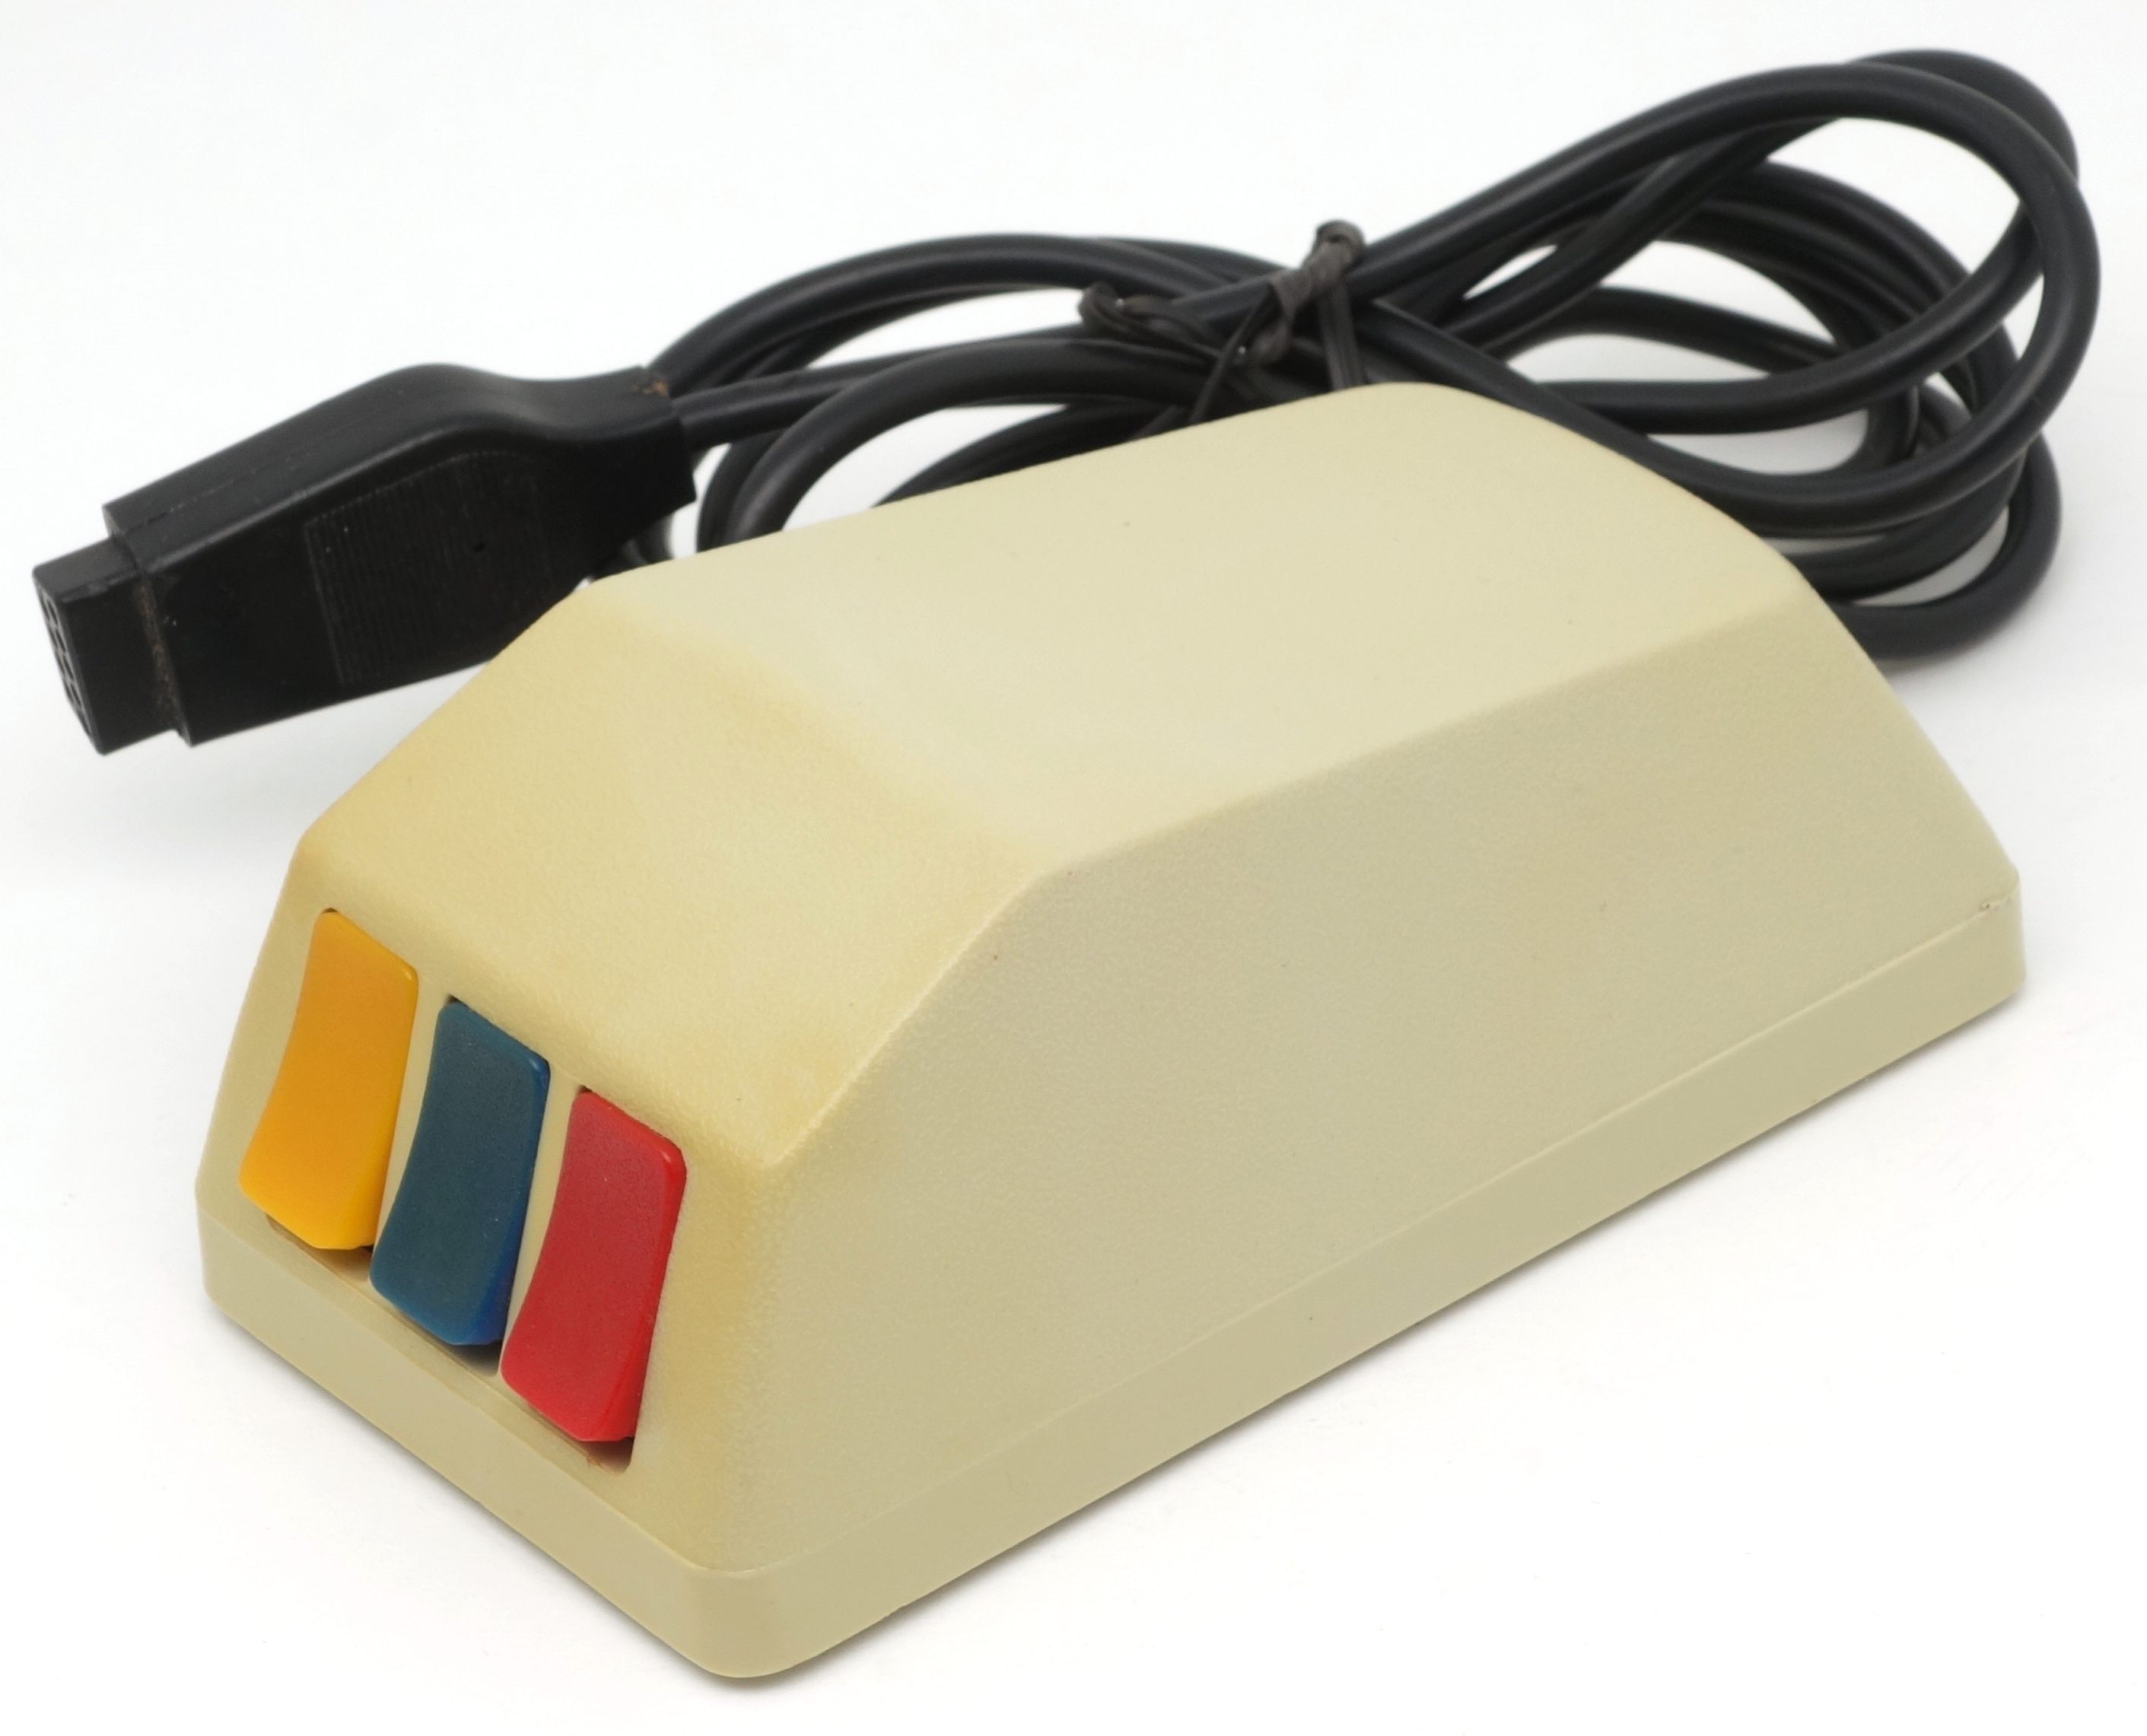
\includegraphics[scale=0.62]{1985_smc_contriver_magic_mouse/pic_30.jpg}
    \caption{Magic Mouse}
    \label{fig:MagicMousePic}
\end{figure}

The mouse is made in a beige case with chopped outlines and has three colored buttons on the inclined front (i.e. the one farthest from the user) side -- red, blue and yellow (fig. \ref{fig:MagicMousePic}). A thick cable comes out from the right side of the case and has a sleeve to protect it from mechanical damage at the exit point. On the bottom side (fig. \ref{fig:MagicMouseTopAndBottom}) there is a large rubber ball located close to the back of the case, a removable ring that allows you to remove it for cleaning the mouse (it is attached with a screw -- a design typical for mice from the first half of the 80s), and two adjustment screws. The screws are used to calibrate so that the pointer can move across the entire screen: the mouse is connected to the analog joystick port and actually emulates it, and the screws play the role of joystick trimmers.

\begin{figure}[h]
    \centering
    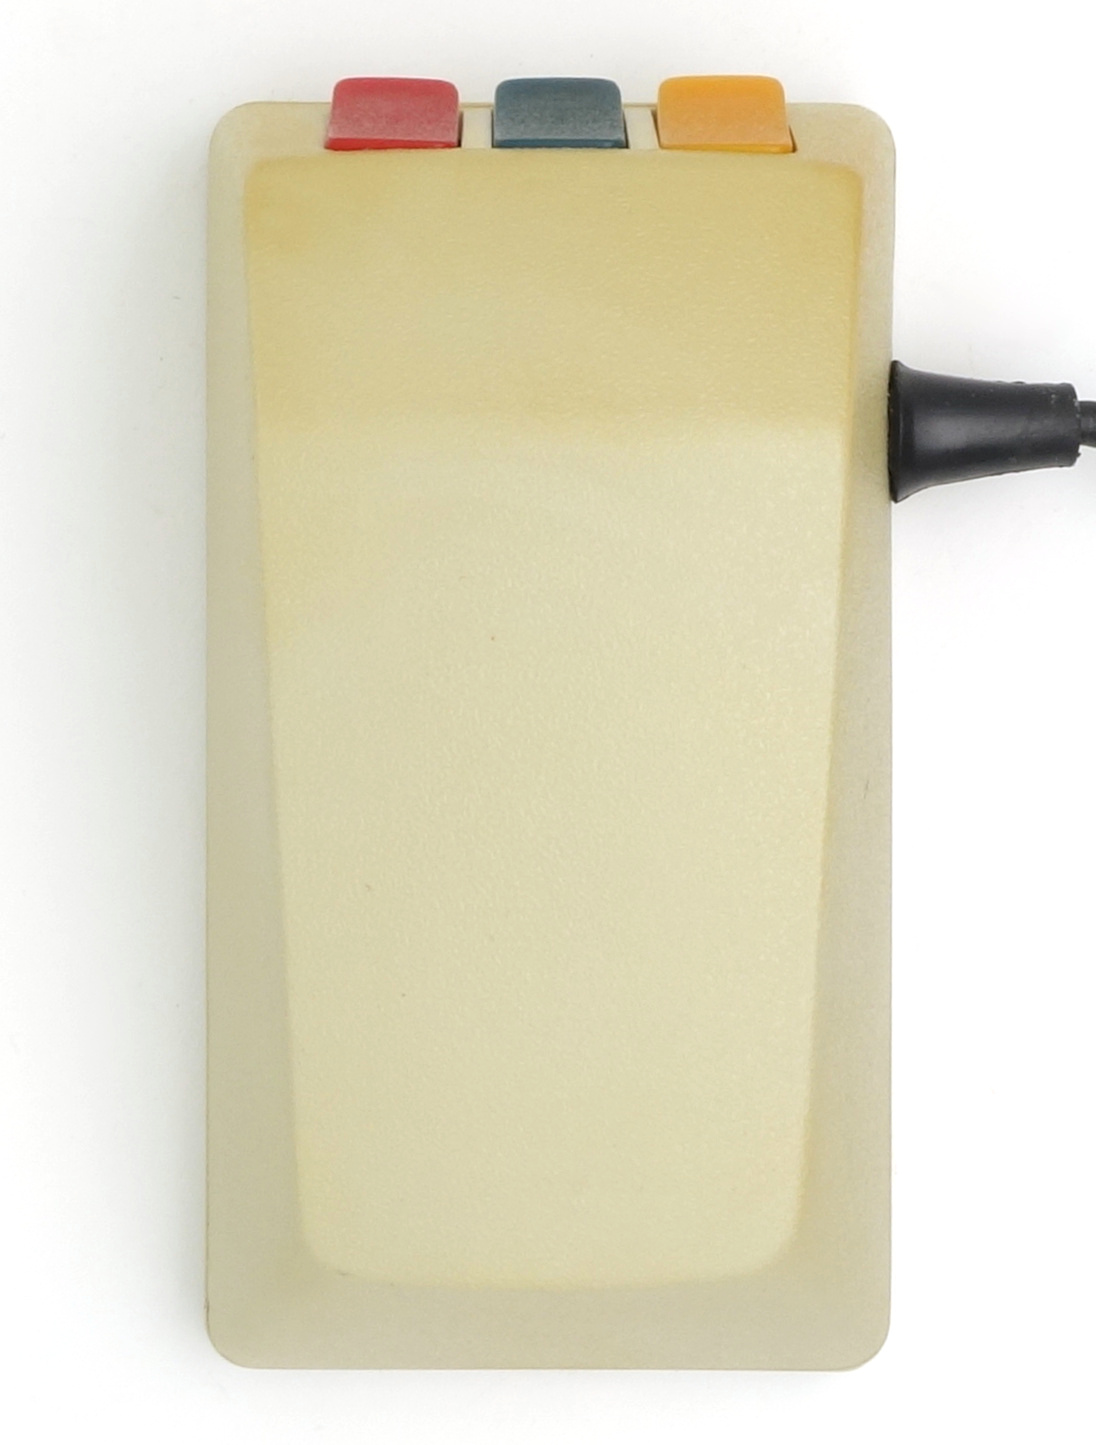
\includegraphics[scale=0.77]{1985_smc_contriver_magic_mouse/top_30.jpg}
    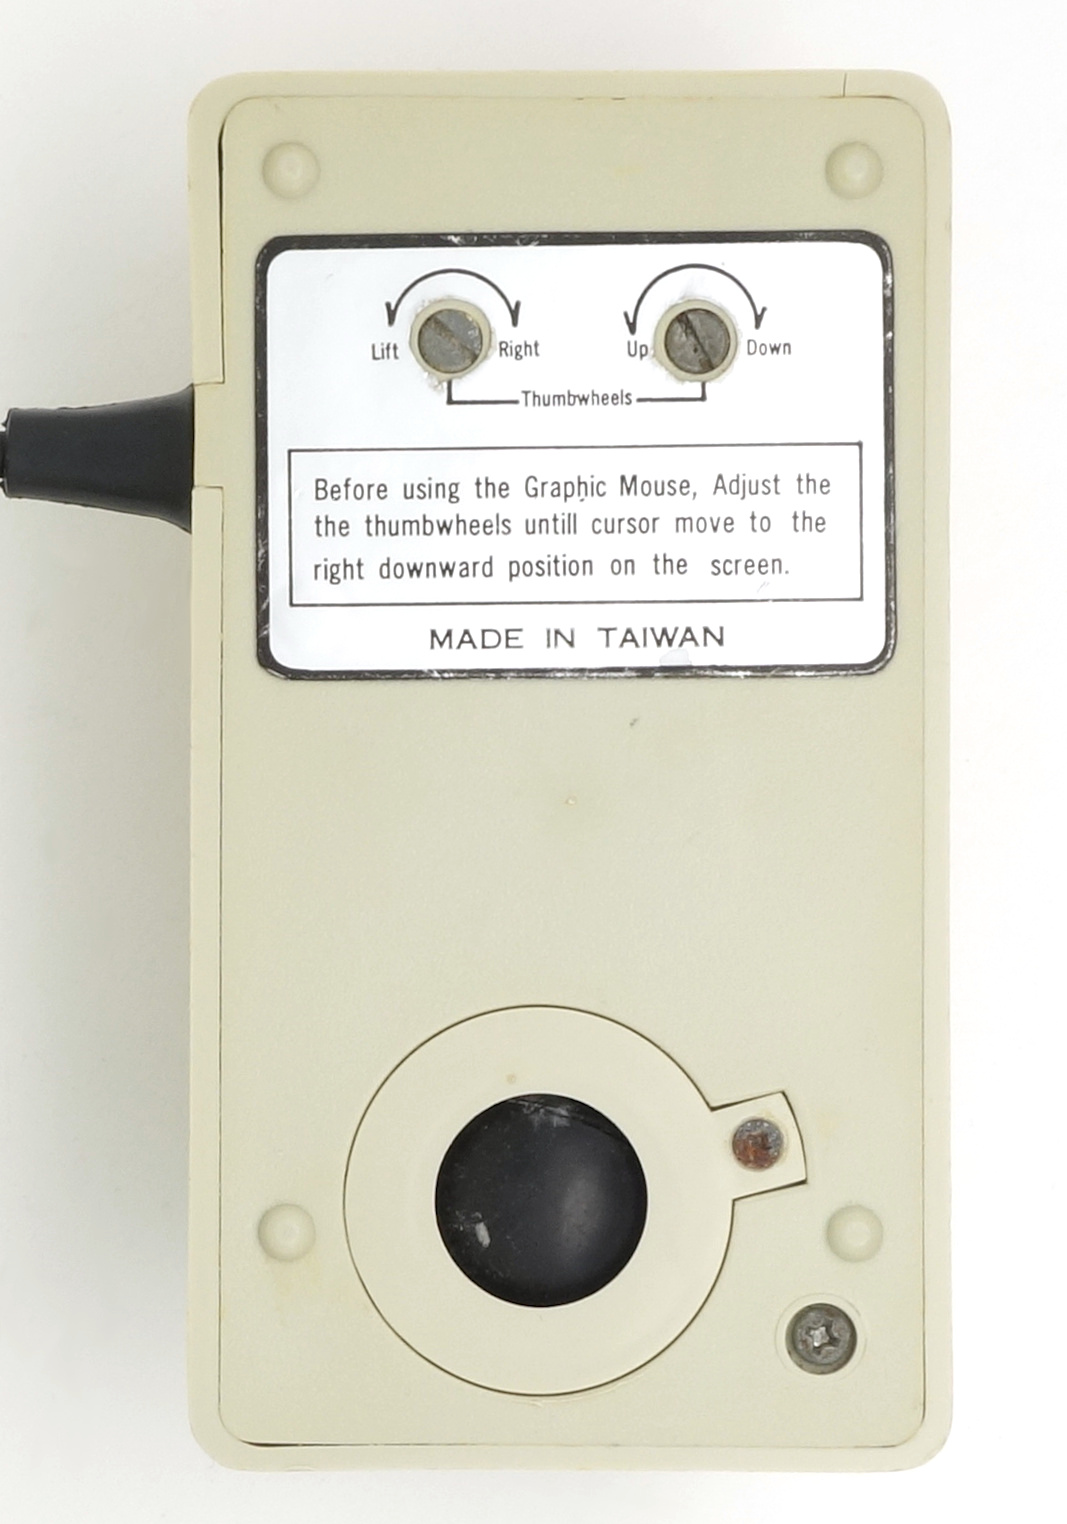
\includegraphics[scale=0.73]{1985_smc_contriver_magic_mouse/bottom_30.jpg}
    \caption{Magic Mouse, top and bottom views}
    \label{fig:MagicMouseTopAndBottom}
\end{figure}

The color differentiation of the buttons apparently goes back to the Xerox mice for the Alto computers, which had color-coded three buttons (Xerox documentation used phrases like ``red mouse click'' and ``yellow mouse click'', which were unfortunate considering that most Alto mice actually had single-color buttons made of gray plastic). The SMC mouse for Commodore is one of the few mice that actually implemented color differentiation of the buttons. The Apple II version of the mouse is made differently: it has a red left button and blue middle and right buttons (and the plastic case has a cooler gray shade).

\begin{figure}[h]
    \centering
    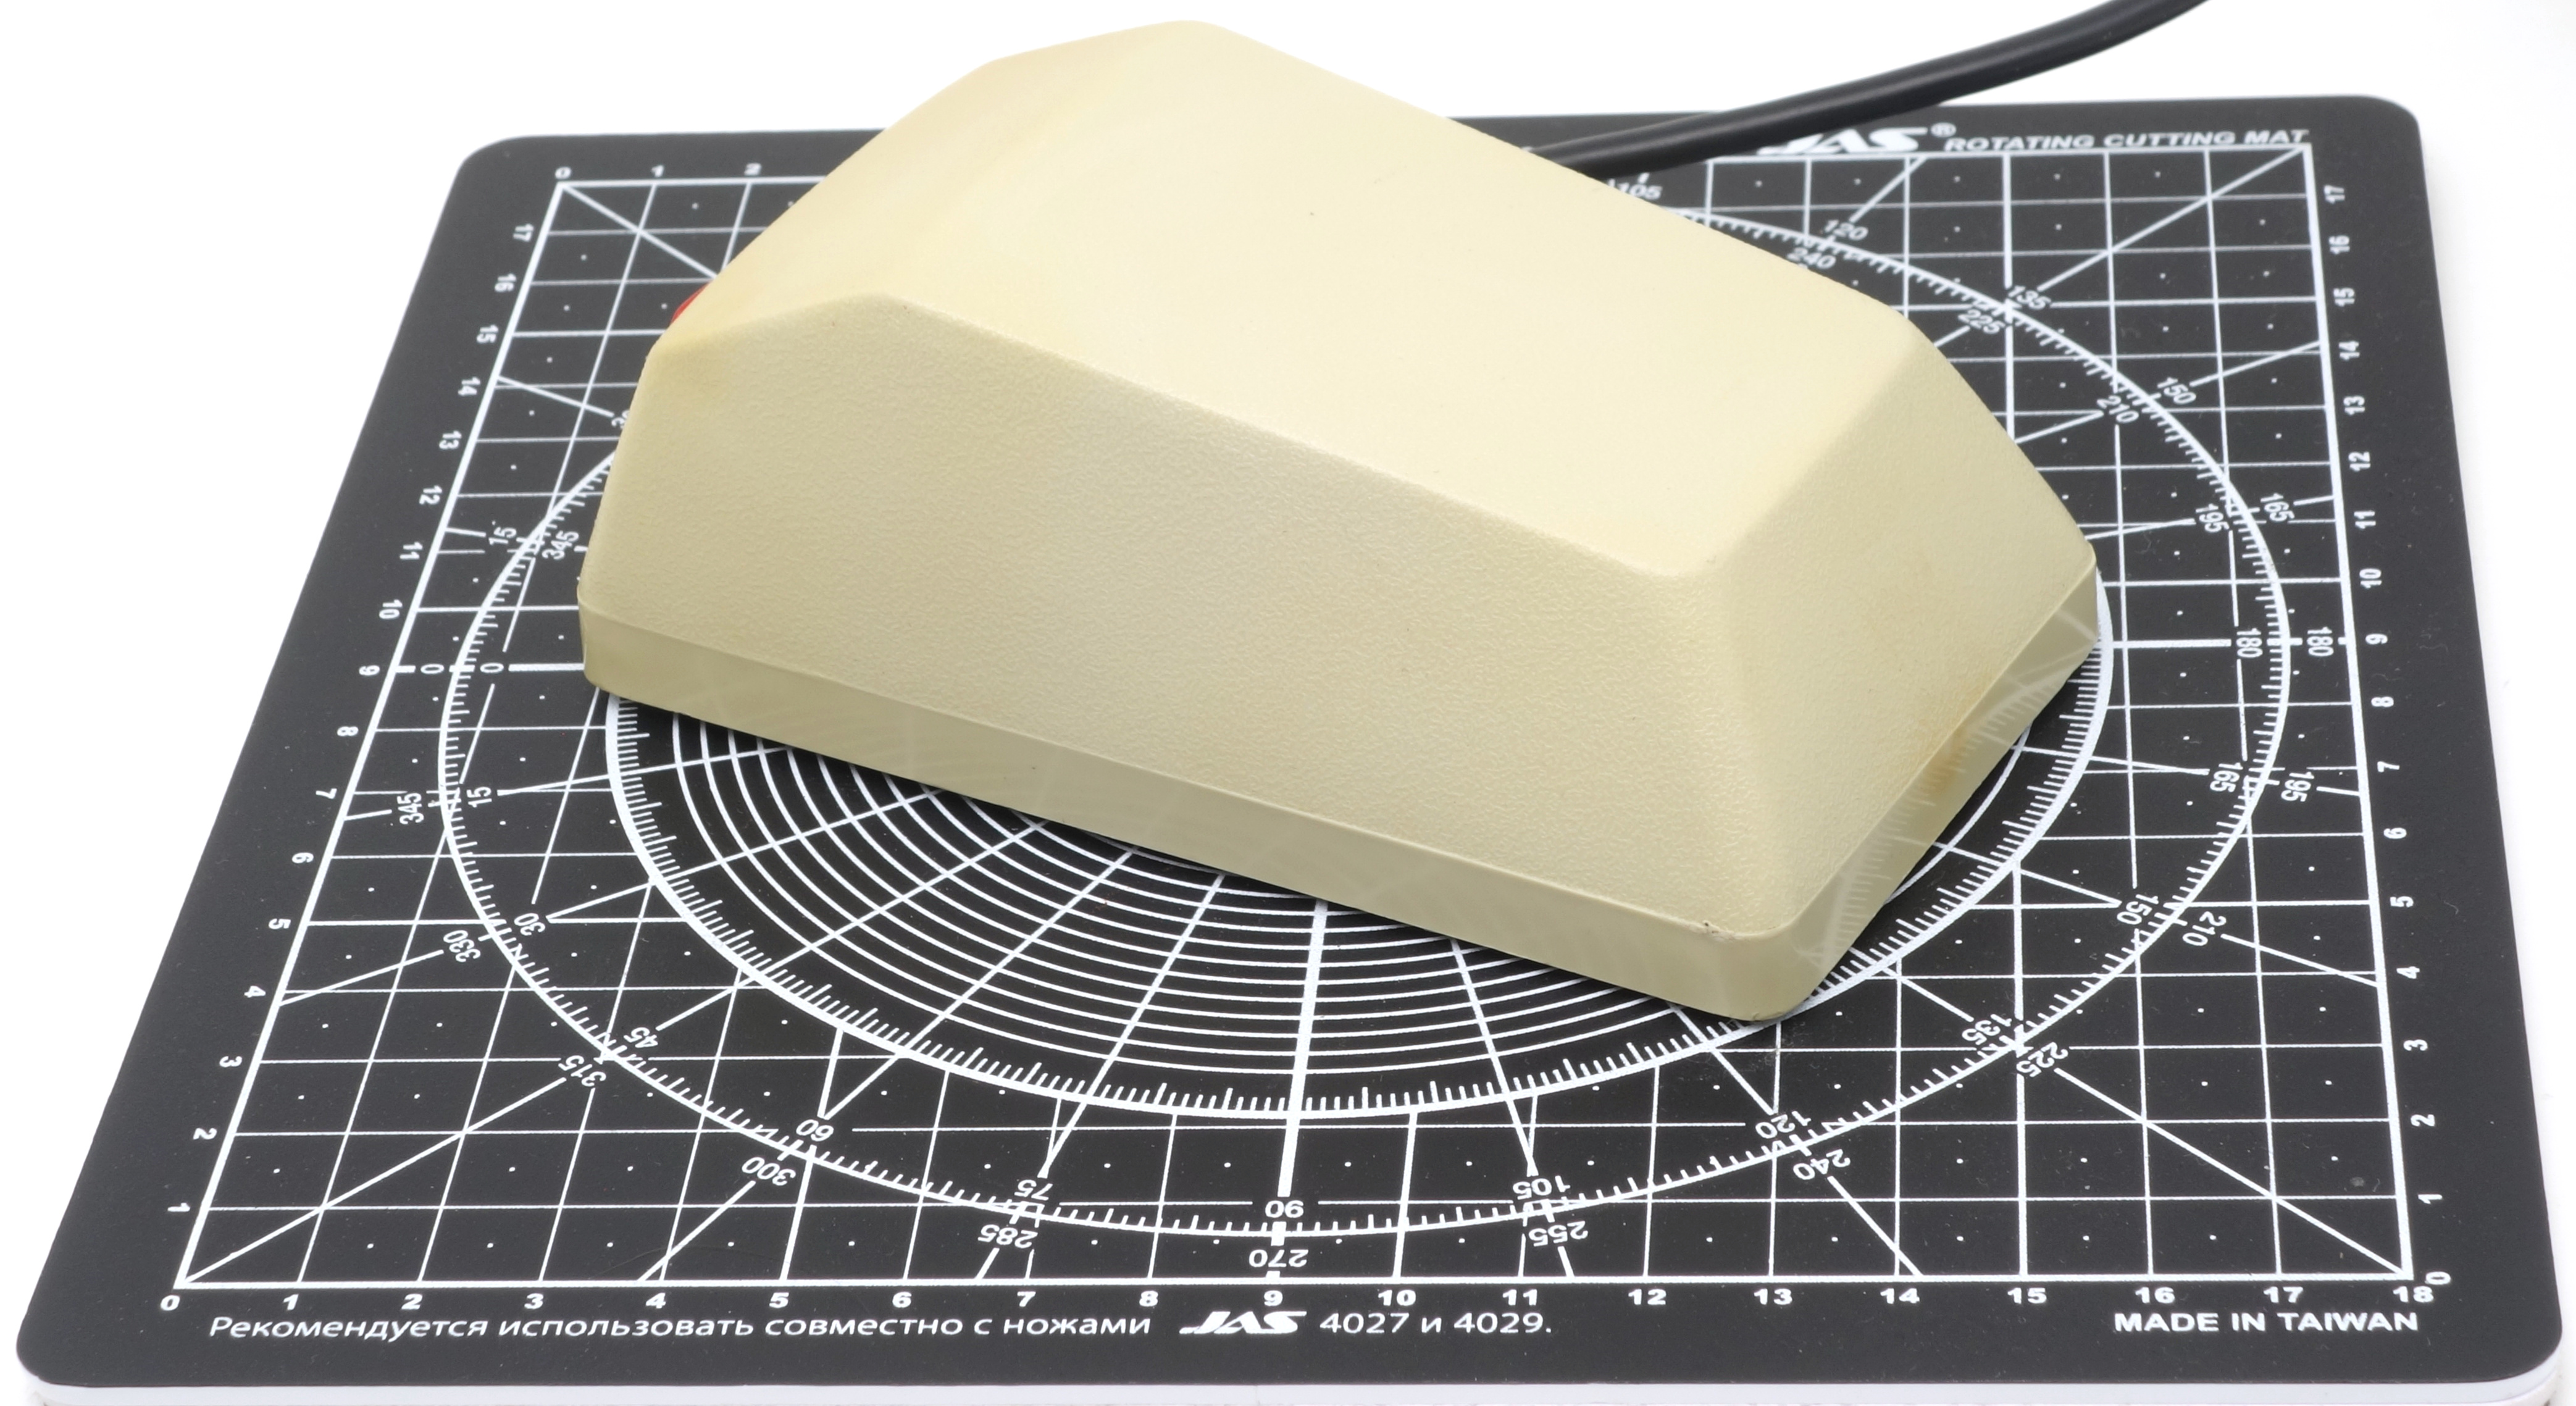
\includegraphics[scale=0.54]{1985_smc_contriver_magic_mouse/size_30.jpg}
    \caption{Magic Mouse on a graduated pad with a grid step of 1~cm}
    \label{fig:MagicMouseSize}
\end{figure}

The mouse is unusually large by 1980s standards (fig. \ref{fig:MagicMouseSize}). Reviewers noted this as the most obvious drawback compared to other mice that fit completely under the palm, along with the mouse's heavy weight \cite{SMC_Mouse_Commodore3}.

The case shape was also considered very inconvenient in reviews. The unfortunate placement of the ball in the user's wrist area (Fig. \ref{fig:MagicMouseHand}) made it even more difficult to control the mouse. In addition, reviewers noted a tremble of the cursor due to the loose fit of the ball, as well as the low resolution of the mouse, which in the programs included with it was only $160 \times 200$ pixels \cite{SMC_Mouse_Commodore3}. At the same time, not a single reviewer mentioned that the vertical arrangement of the buttons creates the possibility of accidentally moving the mouse back when pressing them --- either the likelihood of this was very small due to the weight and size of the mouse, or this drawback was insignificant compared to other problems with its hardware and software. In particular, \cite{SMC_Mouse_Commodore3} notes that the pointer's movements lag behind the user's mouse movements, and their positions become synchronized only after the movement has stopped, which greatly complicates precise positioning. Fine mouse operation turned out to be extremely difficult (in addition to trembling, it is also complicated by the fact that the actual drawn point is slightly higher than the pointer position). Therefore, in the Hi-Res Graphic Designer graphic editor that comes with the mouse, the keyboard keys are used to move the cursor one-pixel in one of eight directions.

\begin{figure}[h]
    \centering
    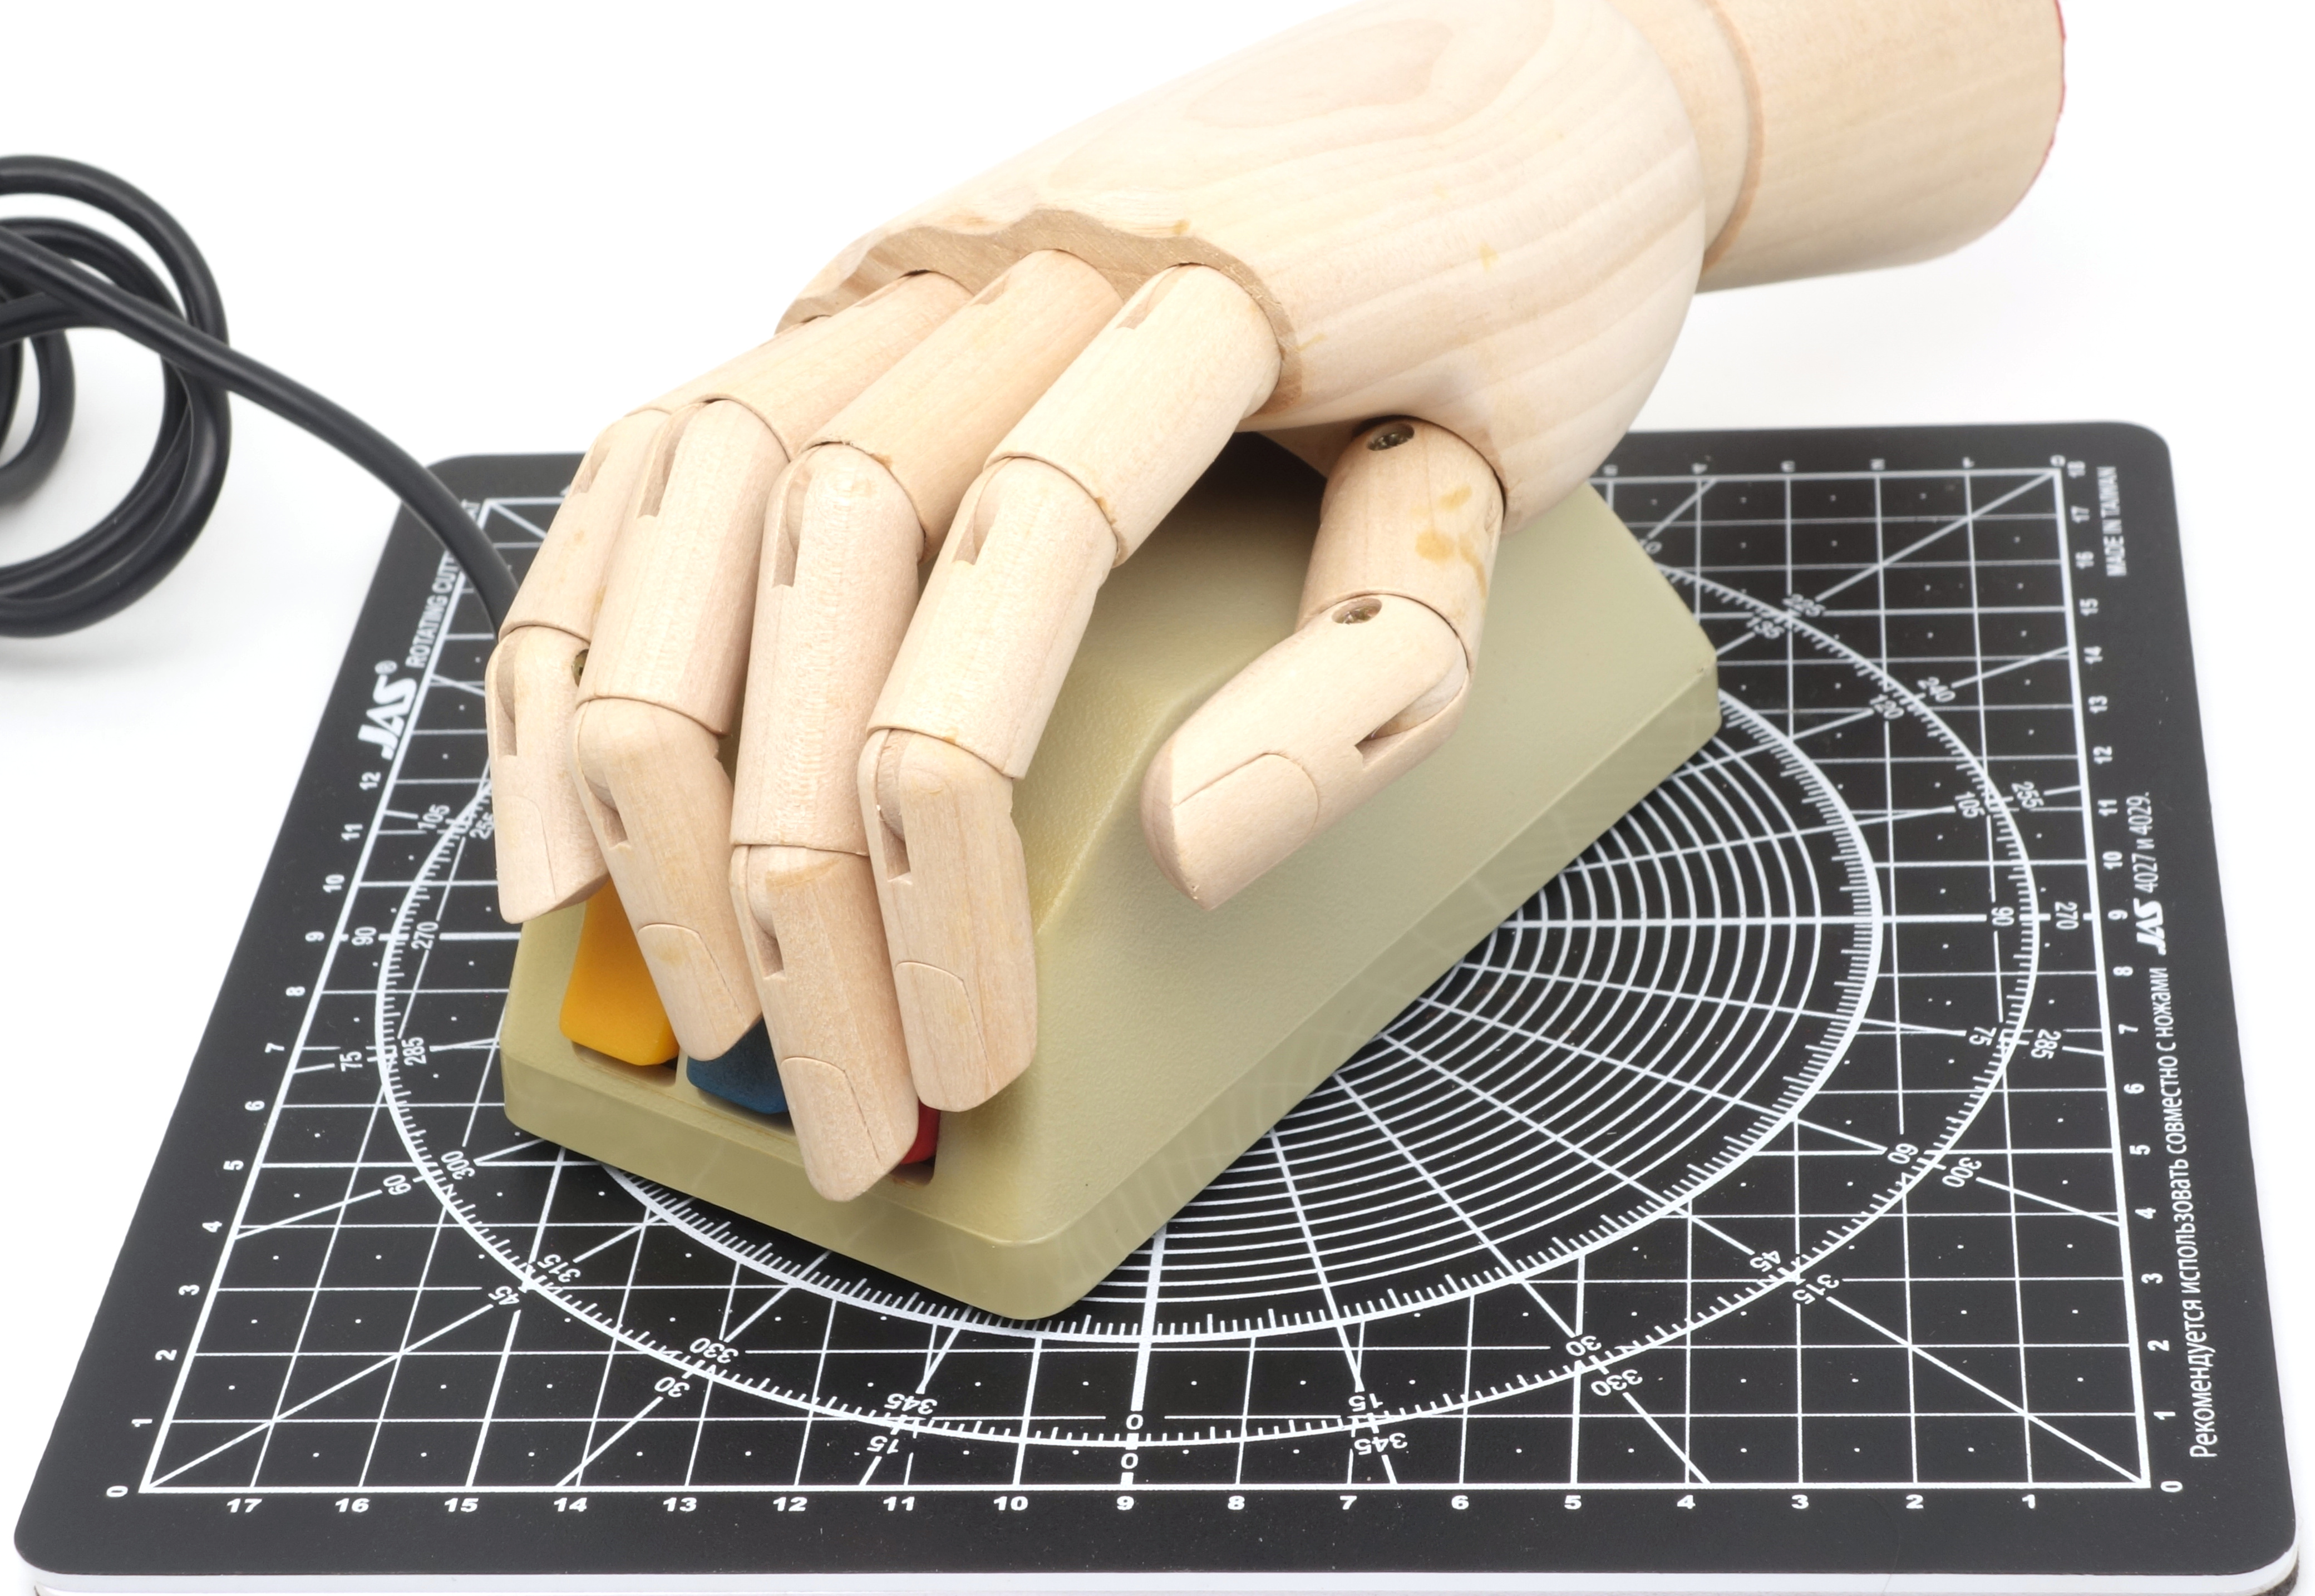
\includegraphics[scale=0.54]{1985_smc_contriver_magic_mouse/hand_30.jpg}
    \caption{Magic Mouse with a human hand model}
    \label{fig:MagicMouseHand}
\end{figure}

An unexpected advantage of the SMC Mouse was its low price: for example, the version for BBC Micro computers, despite its size and weight, cost \pounds 59.95, as opposed to \pounds 89.95 for the standard first-generation AMX mouse with the same configuration. Obviously, the reason was the lower cost due to production in Taiwan, but price dumping is also quite likely.

 \begin{figure}[h]
    \centering
    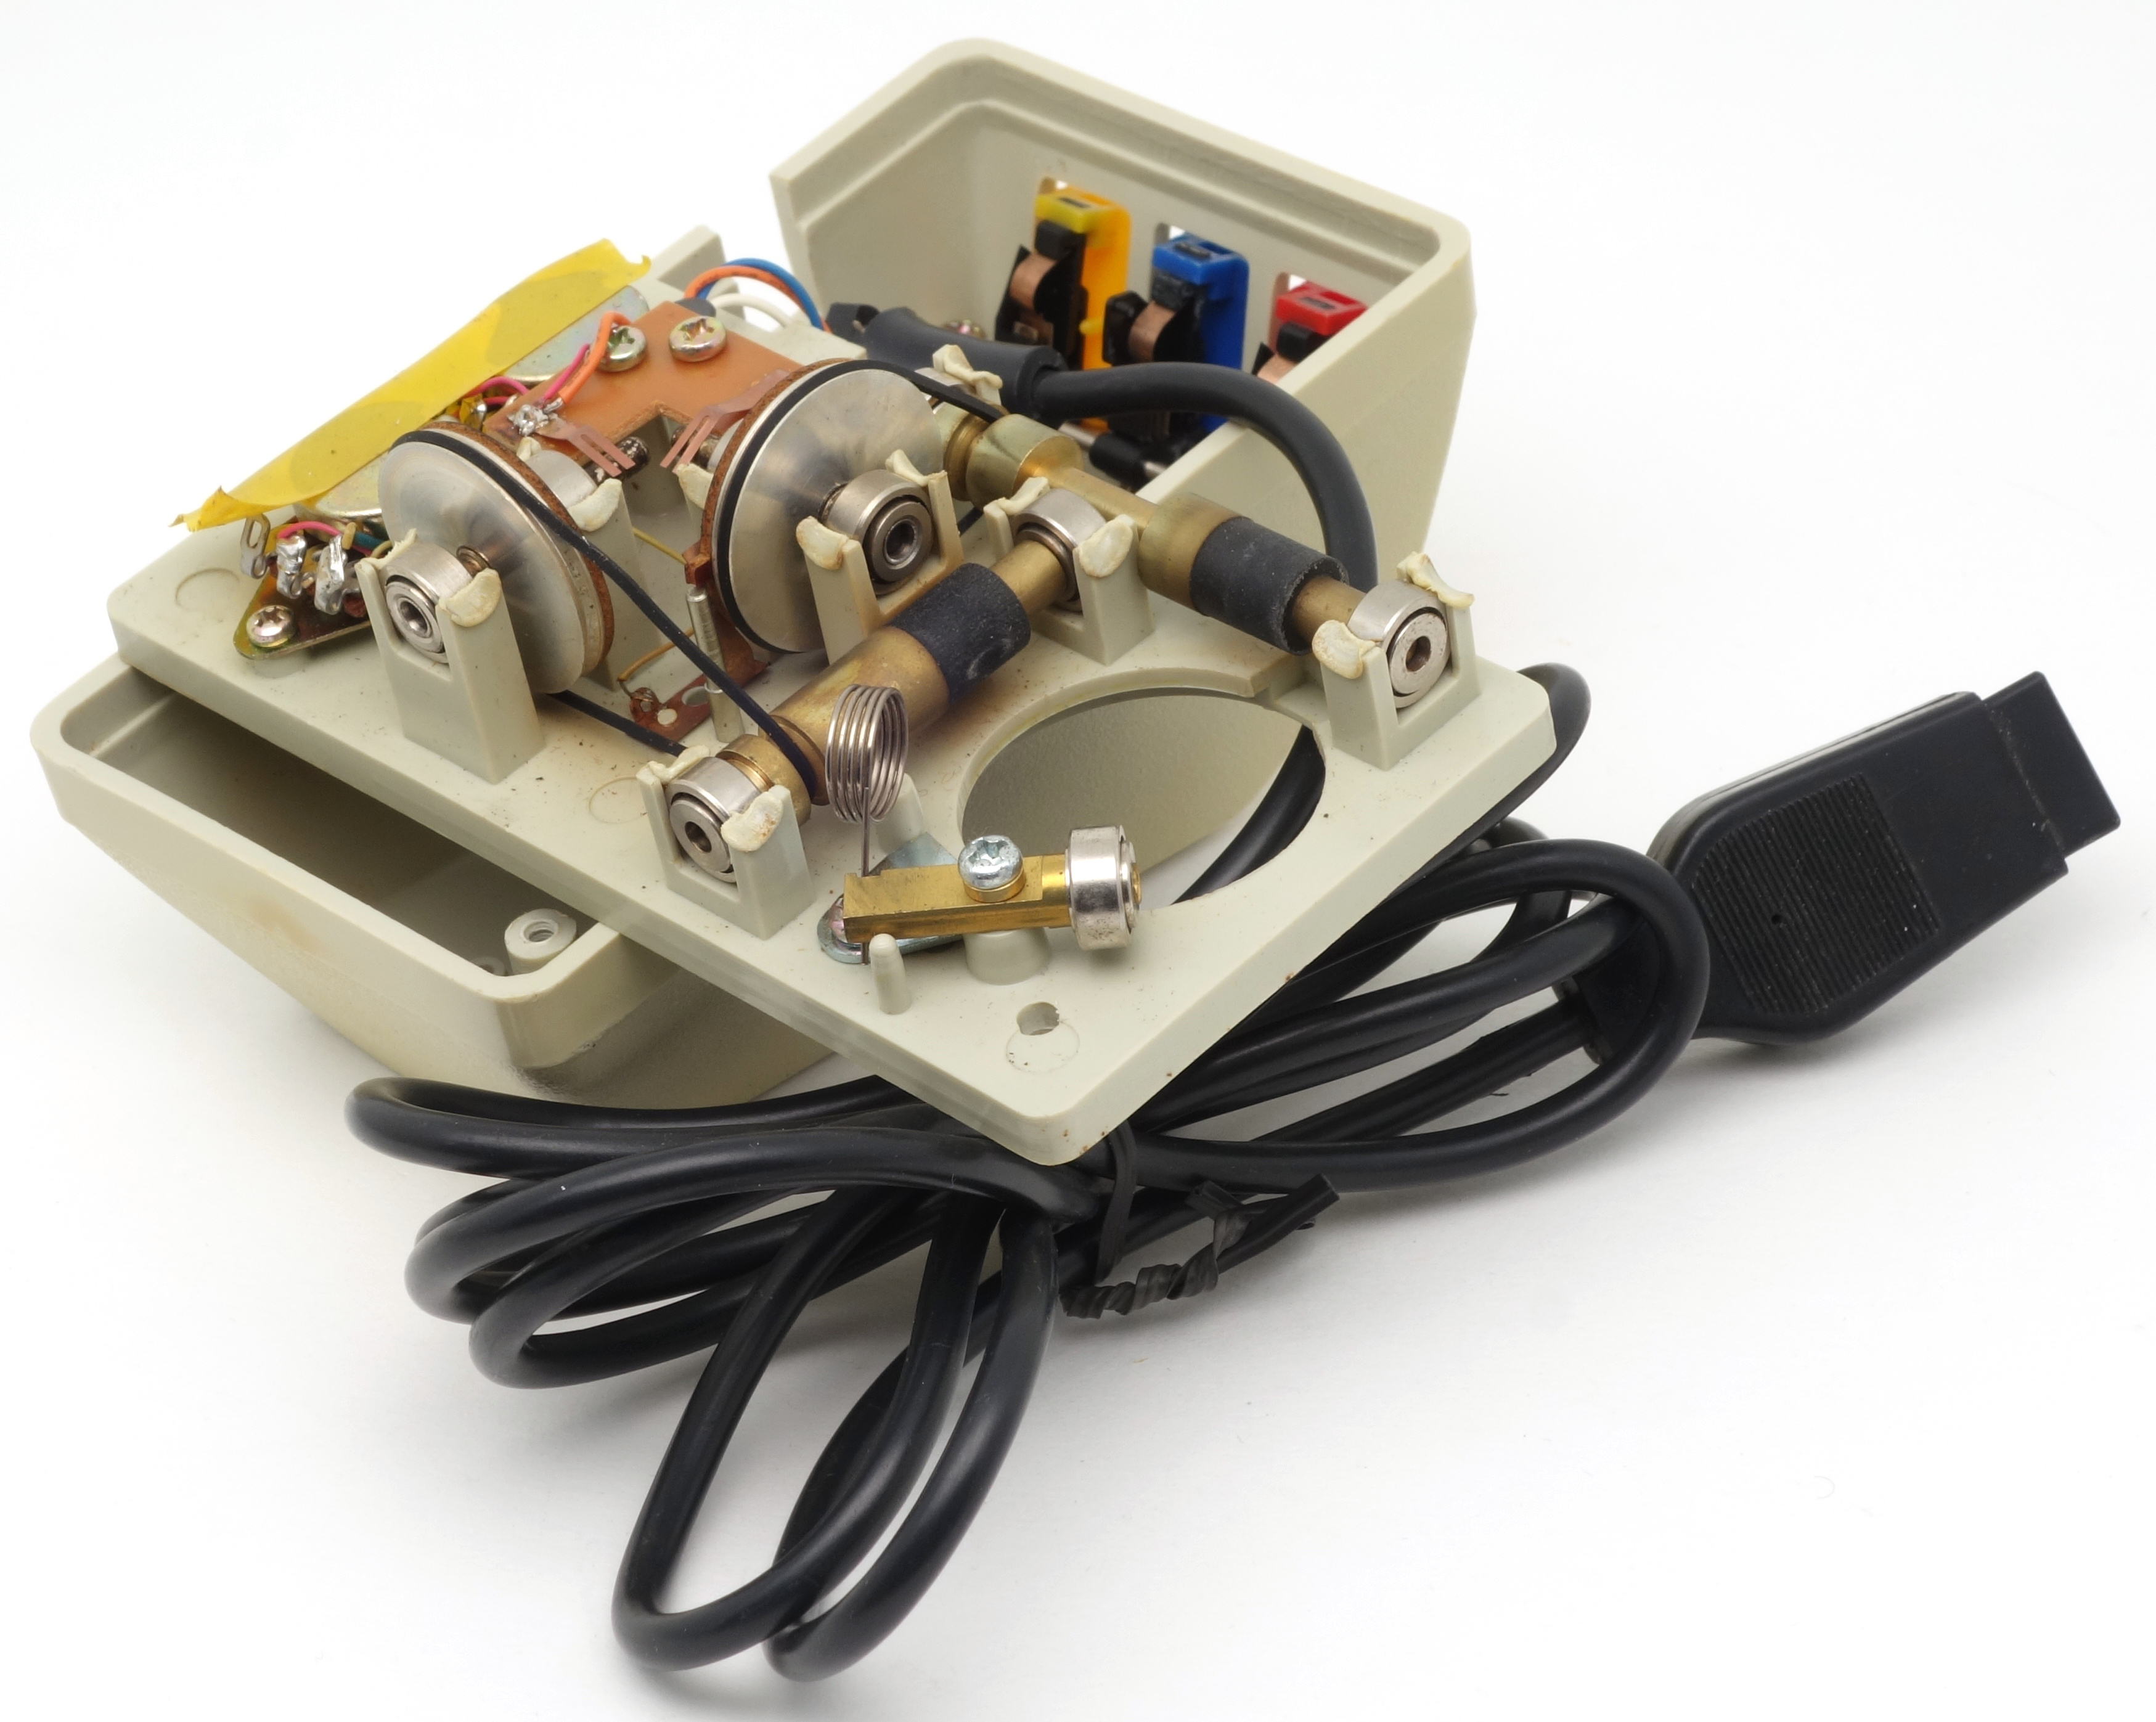
\includegraphics[scale=0.65]{1985_smc_contriver_magic_mouse/inside_30.jpg}
    \caption{Magic Mouse disassembled}
    \label{fig:MagicMouseInside}
\end{figure}


The internal structure of the mouse can be seen in fig. \ref{fig:MagicMouseInside}. As you can see, the rotation of the rollers by the ball when moving the mouse is transmitted via belt drives to two potentiometers. The design involves a significant number of expensive metal parts, the roller axes and potentiometers are mounted on bearings, which does not correspond to the cheap selling price of the product.

~

\begin{thebibliography}{9}
\bibitem{c64wiki} Mouse -- C64-Wiki \url{https://www.c64-wiki.com/wiki/Mouse}
\bibitem {SMC_Mouse_Commodore1} Mouse with graphics // Acorn user, June 1985. -- P. 127 \url{https://archive.org/details/AcornUser035-Jun85/page/n127/mode/2up}
\bibitem {SMC_Mouse_Commodore2} Connor P. Joysticks survey // Your computer, August, 1985. p. 32--34 \url{https://archive.org/details/your-computer-magazine-1985-08/page/n33/mode/2up}
\bibitem {SMC_Mouse_Commodore3} Janda D. Hardware pro-test: SMC Mouse // Personal Computer News, Iss. 107, April 20, 1985. -- P. 32 \url{https://archive.org/details/PersonalComputerNews/PersonalComputerNews107-20Apr1985/page/n33/mode/2up}
\bibitem {CHM} Ideal Magic Mouse. Computer History Museum. \url{https://www.computerhistory.org/collections/catalog/102633276}
\bibitem {reddit} Mice. (and a story!). reddit.com
 \url{https://www.reddit.com/r/retrobattlestations/comments/8ket13/mice_and_a_story/}
\end{thebibliography}
\end{document}
